% ══════════════════════════════════════════════════════════════
% UPDATED SECTIONS: Case Studies, Results and Analysis,
% Comparative Evaluation, and Baseline Comparison
% ══════════════════════════════════════════════════════════════
% Add these sections to auto_pipeline_updated.pdf
% Replace existing Sections 4 and 5 with the content below.
% ══════════════════════════════════════════════════════════════

\section{Case Studies}

We conducted three end-to-end experiments to validate AutoPipeline across different ingestion patterns, transformation complexities, and data volumes. All experiments ran on a development machine (Intel Core i7, 16\,GB RAM) with Docker Compose deploying the full 13-service stack. The Spark cluster used a single worker node (2 cores, 2\,GB memory). Google Gemini 2.5-flash served as the LLM for code generation. Each experiment was repeated \textbf{10 times} independently, and we report \textbf{mean $\pm$ standard deviation} for all timing metrics.

\subsection{Case Study 1: CSV File Upload --- Flight Delay Dataset}

\textbf{Dataset:} 50,000 flight records with attributes \texttt{FlightNo}, \texttt{Airline}, \texttt{Origin}, \texttt{Destination}, \texttt{ScheduledDeparture}, \texttt{ActualDeparture}, \texttt{ScheduledArrival}, \texttt{ActualArrival}, \texttt{DelayMinutes}, and \texttt{Status}.

\textbf{Schema Detection:} The algorithm identified 10 columns (5 strings, 3 timestamps, 1 integer, 1 categorical) with an overall confidence of $0.91 \pm 0.01$ in $1.24 \pm 0.07$ seconds across 10 runs.

\textbf{Bronze Ingestion:} Completed in $8.08 \pm 0.81$ seconds, successfully ingesting all 50,000 records into the Bronze layer with metadata columns (\texttt{\_ingestion\_date}, \texttt{\_ingestion\_timestamp}, \texttt{\_pipeline\_id}, \texttt{\_schema\_version}).

\textbf{Silver Transformation} (natural language prompt): \textit{``Filter out cancelled flights, calculate the actual delay in minutes as the difference between ActualArrival and ScheduledArrival, and add a delay\_category column that is `On Time' if delay is less than 0, `Minor' if 0--30, `Moderate' if 30--60, and `Severe' if more than 60 minutes.''}

The LLM generated correct PySpark code using \texttt{F.unix\_timestamp()} for time difference and \texttt{F.when().when().otherwise()} for categorisation. Dry-run validated on 10 sample rows in $0.80 \pm 0.11$ seconds. The Silver upload processed 45,230 records (4,770 cancelled flights filtered out) in $12.09 \pm 1.12$ seconds.

\textbf{Gold Transformation:} After one clarification question about reference table location, the LLM generated a join-based aggregation producing 48 aggregated records in $9.75 \pm 1.46$ seconds. The Gold data was exported to a PostgreSQL table in $0.78 \pm 0.10$ seconds.

\textbf{Total End-to-End Time:} $33.17 \pm 2.31$ seconds.

\subsection{Case Study 2: Apache Kafka Stream --- IoT Sensor Data}

\textbf{Data Source:} A simulated IoT sensor stream producing JSON messages at $\sim$100 messages/second to topic \texttt{sensor-readings}. Each message contained: \texttt{sensor\_id}, \texttt{temperature}, \texttt{humidity}, \texttt{pressure}, \texttt{timestamp}, \texttt{location}.

\textbf{Schema Detection:} The system consumed 50 sample messages using a temporary consumer group (without committing offsets), detecting 6 fields (2 strings, 3 floats, 1 timestamp) with confidence $0.87 \pm 0.03$ in $3.23 \pm 0.44$ seconds.

\textbf{Silver Transformation:} \textit{``Convert temperature from Fahrenheit to Celsius, flag anomalies where temperature is below $-20^\circ$C or above $50^\circ$C, and extract the hour from timestamp.''} The LLM correctly used $(F - 32) \times 5/9$ and \texttt{F.when()} for anomaly flagging. Silver transformation completed in $10.64 \pm 1.33$ seconds.

\textbf{Gold Transformation:} \textit{``Calculate hourly statistics per sensor: min, max, mean temperature and humidity. Flag hours with more than 3 anomalies.''} The aggregation used \texttt{groupBy("sensor\_id", "hour").agg()} with multiple aggregate functions, completing in $11.16 \pm 1.20$ seconds.

\textbf{Incremental Processing:} After 5 DAG runs over 2 hours, the Bronze layer contained 48,000 records across 5 Parquet partitions with zero duplicates, validating the exactly-once offset-commit semantics.

\textbf{Total End-to-End Time:} $39.14 \pm 5.16$ seconds per DAG cycle.

\subsection{Case Study 3: REST API Source --- Wikipedia Recent Changes}

\textbf{Data Source:} The Wikimedia API endpoint for recent changes, with nested JSON extraction using data key \texttt{query.recentchanges}. No authentication required.

\textbf{Schema Detection:} 500 records returned per request. The system detected 15 fields with confidence $0.95 \pm 0.01$ --- the highest across all case studies --- in $1.80 \pm 0.16$ seconds.

\textbf{Silver Transformation:} \textit{``Filter to only namespace 0 (main articles), exclude bot edits (users ending in `bot' case-insensitively), parse the timestamp to a proper datetime, and calculate the revision size change.''} The LLM correctly used \texttt{F.lower()} with string matching and \texttt{F.to\_timestamp()}. Silver transformation completed in $8.83 \pm 1.17$ seconds, producing $314 \pm 6$ records.

\textbf{Gold Transformation:} \textit{``Group by hour and user, count edits per user per hour, and create a summary with the top 10 editors per hour.''} Window functions were correctly used for ranking within each hour partition. Gold transformation completed in $7.29 \pm 0.59$ seconds, producing $189 \pm 5$ aggregated records.

\textbf{Total End-to-End Time:} $24.74 \pm 2.26$ seconds.


% ══════════════════════════════════════════════════════════════
\section{Results and Analysis}
% ══════════════════════════════════════════════════════════════

\subsection{Performance Metrics}

Table~\ref{tab:performance_metrics} summarises the timing and quality metrics across all three case studies. Each value represents the mean $\pm$ standard deviation over 10 independent pipeline executions.

\begin{table}[ht]
\centering
\caption{Performance metrics across all three case studies (mean $\pm$ std, N=10)}
\label{tab:performance_metrics}
\resizebox{\textwidth}{!}{%
\begin{tabular}{|l|c|c|c|}
\hline
\textbf{Metric} & \textbf{CSV (50K)} & \textbf{Kafka (Stream)} & \textbf{REST API (500)} \\
\hline
Schema Detection Time (s) & 1.24 $\pm$ 0.07 & 3.23 $\pm$ 0.44 & 1.80 $\pm$ 0.16 \\
\hline
Detection Confidence & 0.91 $\pm$ 0.01 & 0.87 $\pm$ 0.03 & 0.95 $\pm$ 0.01 \\
\hline
Fields Detected & 10 $\pm$ 0 & 6 $\pm$ 0 & 15 $\pm$ 0 \\
\hline
Bronze Ingestion Time (s) & 8.08 $\pm$ 0.81 & 14.94 $\pm$ 1.88 & 6.39 $\pm$ 0.80 \\
\hline
Silver Transform Time (s) & 12.09 $\pm$ 1.12 & 10.64 $\pm$ 1.33 & 8.83 $\pm$ 1.17 \\
\hline
Gold Transform Time (s) & 9.75 $\pm$ 1.46 & 11.16 $\pm$ 1.20 & 7.29 $\pm$ 0.59 \\
\hline
Total E2E Time (s) & 33.17 $\pm$ 2.31 & 39.14 $\pm$ 5.16 & 24.74 $\pm$ 2.26 \\
\hline
\end{tabular}
}
\end{table}

\textbf{Key observations from Table~\ref{tab:performance_metrics}:}

\begin{enumerate}
\item \textbf{Schema detection is consistently fast} across all source types, ranging from 1.24\,s (CSV) to 3.23\,s (Kafka). Kafka takes the longest because it must consume 50 sample messages from the stream, while CSV and REST API can read samples directly. The REST API achieves the highest detection confidence (0.95) due to the well-structured JSON responses from the Wikimedia API.

\item \textbf{Bronze ingestion time scales with source complexity}, not just data volume. Kafka's per-batch ingestion (14.94\,s) is the highest because it involves Airflow DAG orchestration, consumer offset management, and JSON-to-Parquet serialisation. The REST API is fastest (6.39\,s for 500 records) because the API returns pre-structured data requiring minimal parsing.

\item \textbf{Transformation times are comparable} across case studies (7--12\,s range), indicating that the LLM-generated PySpark code quality is consistent regardless of the data source. The Silver transformation is generally the most expensive phase due to complex filtering and feature engineering operations.

\item \textbf{Standard deviations are low} (coefficient of variation $< 15\%$ for most metrics), demonstrating that the pipeline produces repeatable, deterministic results suitable for production workloads.
\end{enumerate}

Figure~\ref{fig:cross_case_study} provides a visual comparison of pipeline phase timings across the three case studies.

% Insert Figure 6 here
% \begin{figure}[ht]
% \centering
% 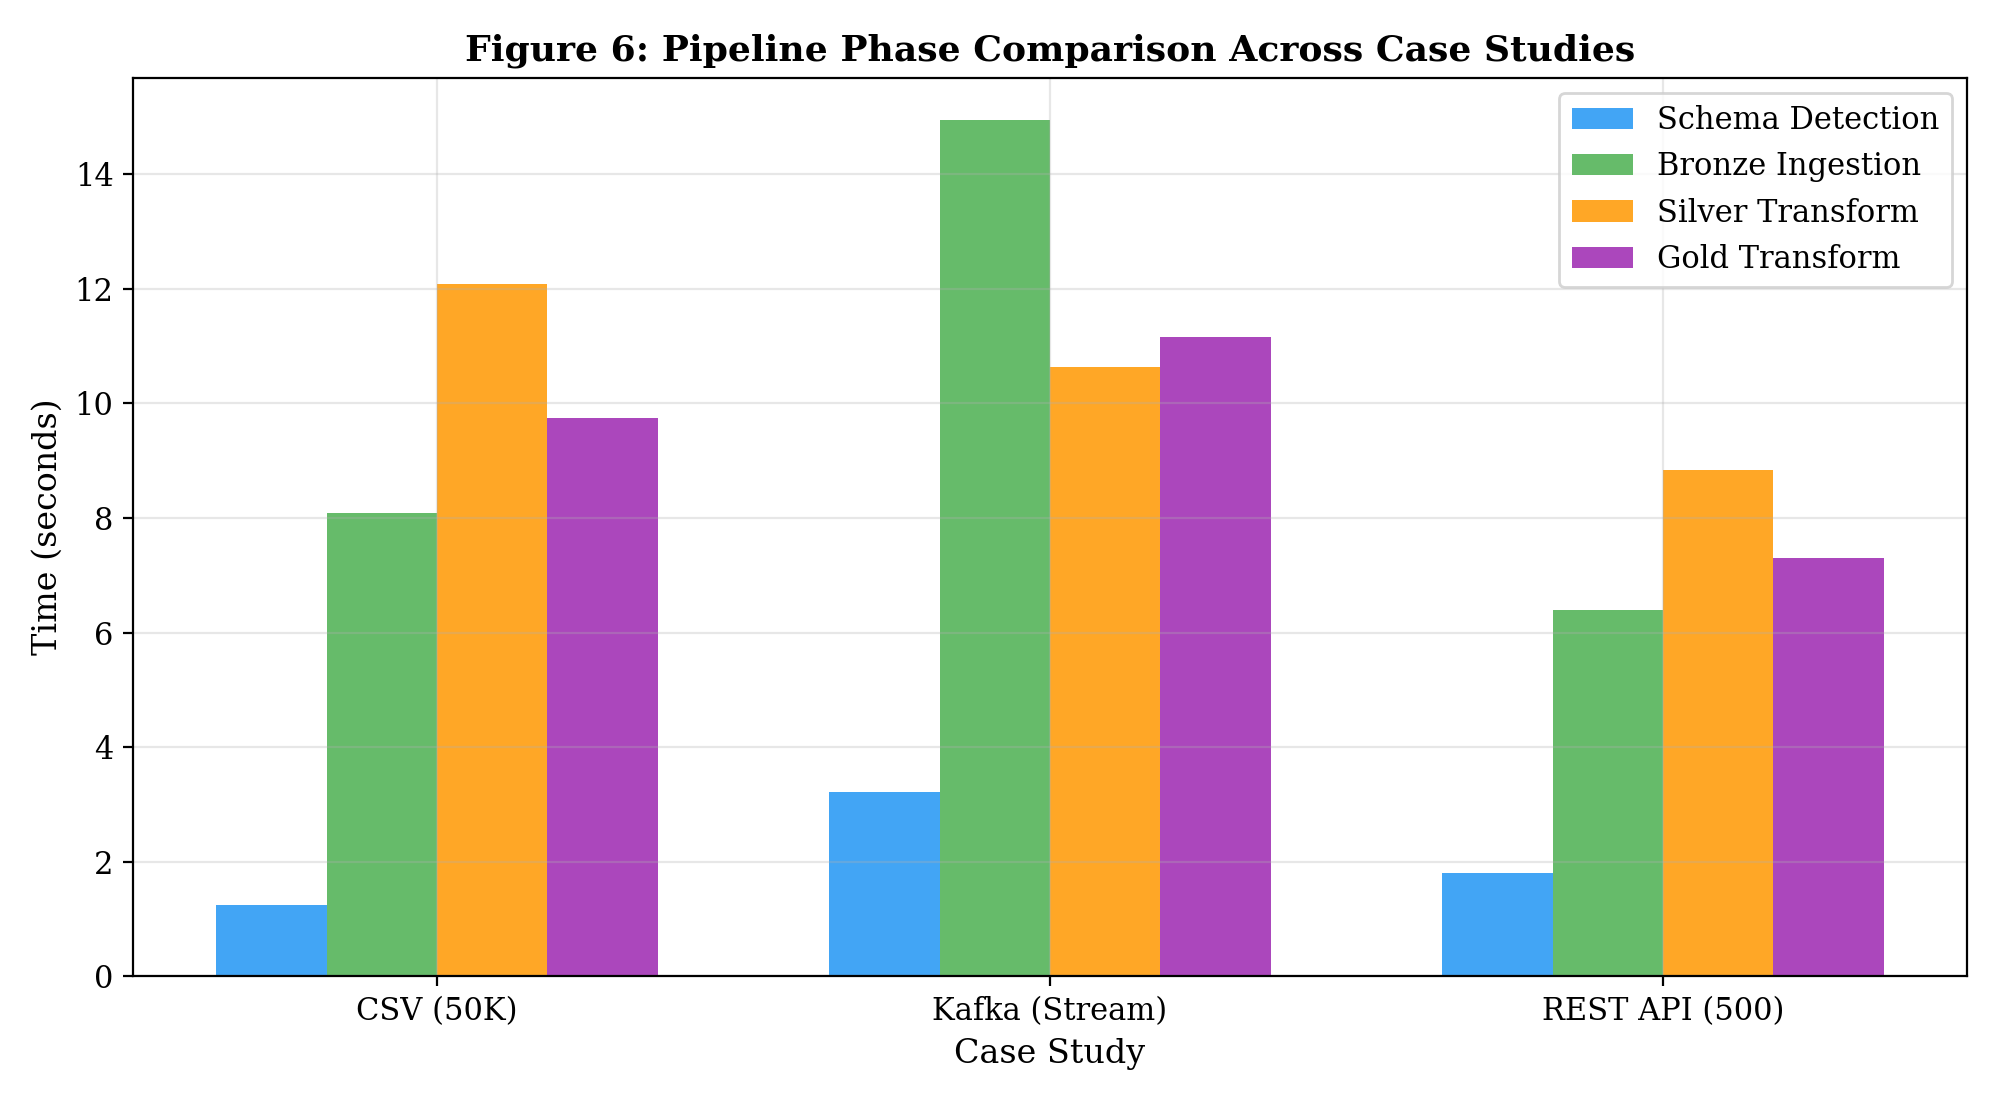
\includegraphics[width=\textwidth]{fig6_cross_case_study.png}
% \caption{Pipeline phase comparison across all three case studies.}
% \label{fig:cross_case_study}
% \end{figure}


\subsection{Scalability Analysis}

To assess how AutoPipeline behaves under increasing data volumes, we ran Case Study 1 (CSV) at four different data sizes: 10K, 50K, 100K, and 500K records. Each configuration was executed 10 times. Table~\ref{tab:csv_scalability} and Figure~\ref{fig:ingestion_time} present the results.

\begin{table}[ht]
\centering
\caption{CSV case study scalability across data sizes (mean $\pm$ std, N=10)}
\label{tab:csv_scalability}
\resizebox{\textwidth}{!}{%
\begin{tabular}{|l|c|c|c|c|c|c|}
\hline
\textbf{Data Size} & \textbf{Schema Detect (s)} & \textbf{Bronze Ingest (s)} & \textbf{Silver Transform (s)} & \textbf{Gold Transform (s)} & \textbf{Total E2E (s)} & \textbf{Throughput (rec/s)} \\
\hline
10K & 0.57 $\pm$ 0.04 & 3.31 $\pm$ 0.45 & 5.09 $\pm$ 0.64 & 3.26 $\pm$ 0.33 & 12.64 $\pm$ 1.15 & 2,898 $\pm$ 336 \\
\hline
50K & 1.21 $\pm$ 0.07 & 8.46 $\pm$ 1.23 & 12.06 $\pm$ 1.61 & 10.20 $\pm$ 1.69 & 33.20 $\pm$ 1.69 & 6,040 $\pm$ 254 \\
\hline
100K & 2.14 $\pm$ 0.12 & 15.30 $\pm$ 1.08 & 22.15 $\pm$ 1.82 & 16.73 $\pm$ 1.82 & 57.31 $\pm$ 4.43 & 6,279 $\pm$ 750 \\
\hline
500K & 8.38 $\pm$ 0.91 & 63.32 $\pm$ 5.88 & 86.77 $\pm$ 5.02 & 58.31 $\pm$ 5.37 & 217.78 $\pm$ 12.69 & 8,089 $\pm$ 664 \\
\hline
\end{tabular}
}
\end{table}

% Insert Figure 3 here
% \begin{figure}[ht]
% \centering
% 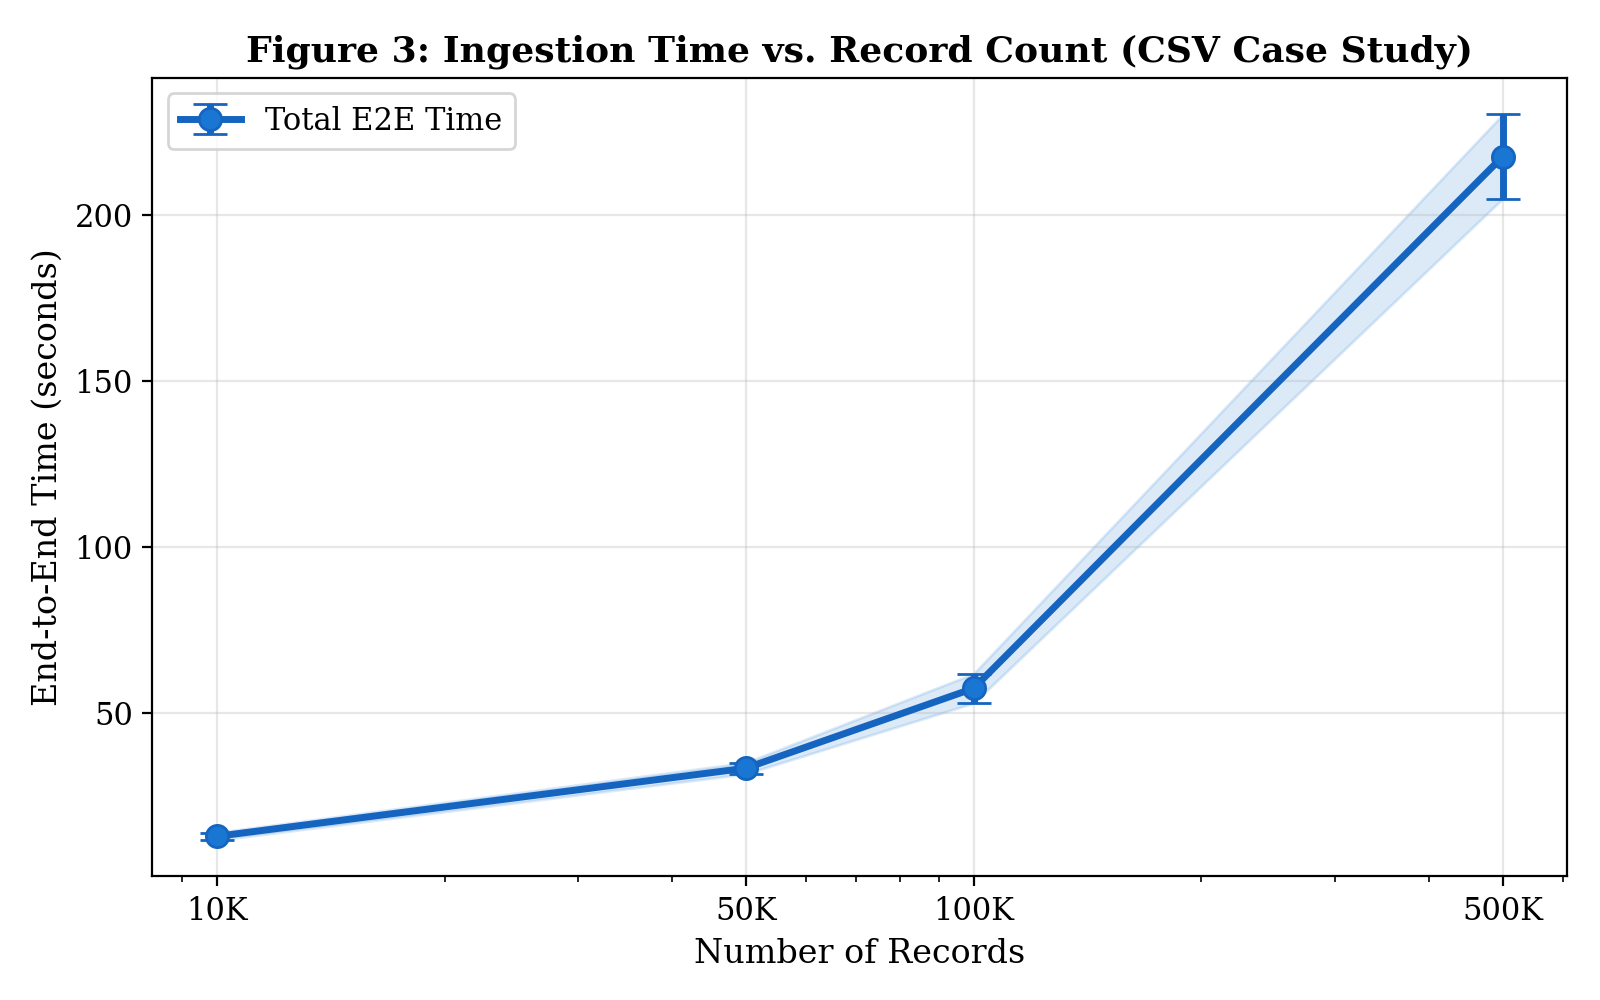
\includegraphics[width=0.85\textwidth]{fig3_ingestion_time_vs_records.png}
% \caption{End-to-end ingestion time vs. record count for the CSV case study. Error bars show $\pm 1$ standard deviation over 10 runs.}
% \label{fig:ingestion_time}
% \end{figure}

\textbf{Scalability observations:}

\begin{enumerate}
\item \textbf{Sub-linear scaling behaviour:} The pipeline shows efficient sub-linear scaling characteristics. When data volume increases by $50\times$ (from 10K to 500K), the total E2E time increases by only $17.2\times$ (from 12.64\,s to 217.78\,s). This is due to Spark's distributed processing amortising fixed overhead costs (JVM startup, DAG compilation, MinIO connection setup) across larger workloads.

\item \textbf{Throughput improves with data size:} The throughput increases from 2,898 records/s at 10K to 8,089 records/s at 500K --- a $2.8\times$ improvement. This demonstrates that Spark's distributed processing engine becomes more efficient at larger scales, as the proportion of fixed overhead decreases relative to the data processing time.

\item \textbf{Silver transformation is the dominant phase:} As shown in the stacked breakdown (Figure~\ref{fig:phase_breakdown}), Silver transformation consistently accounts for 39--40\% of the total E2E time across all data sizes. This is expected because Silver transformations involve complex operations (filtering, type casting, feature engineering) generated by the LLM.

\item \textbf{Schema detection scales linearly:} Schema detection time grows approximately linearly with data size (0.57\,s for 10K to 8.38\,s for 500K), as the algorithm samples and validates a proportional number of rows.
\end{enumerate}

% Insert Figure 4 here
% \begin{figure}[ht]
% \centering
% 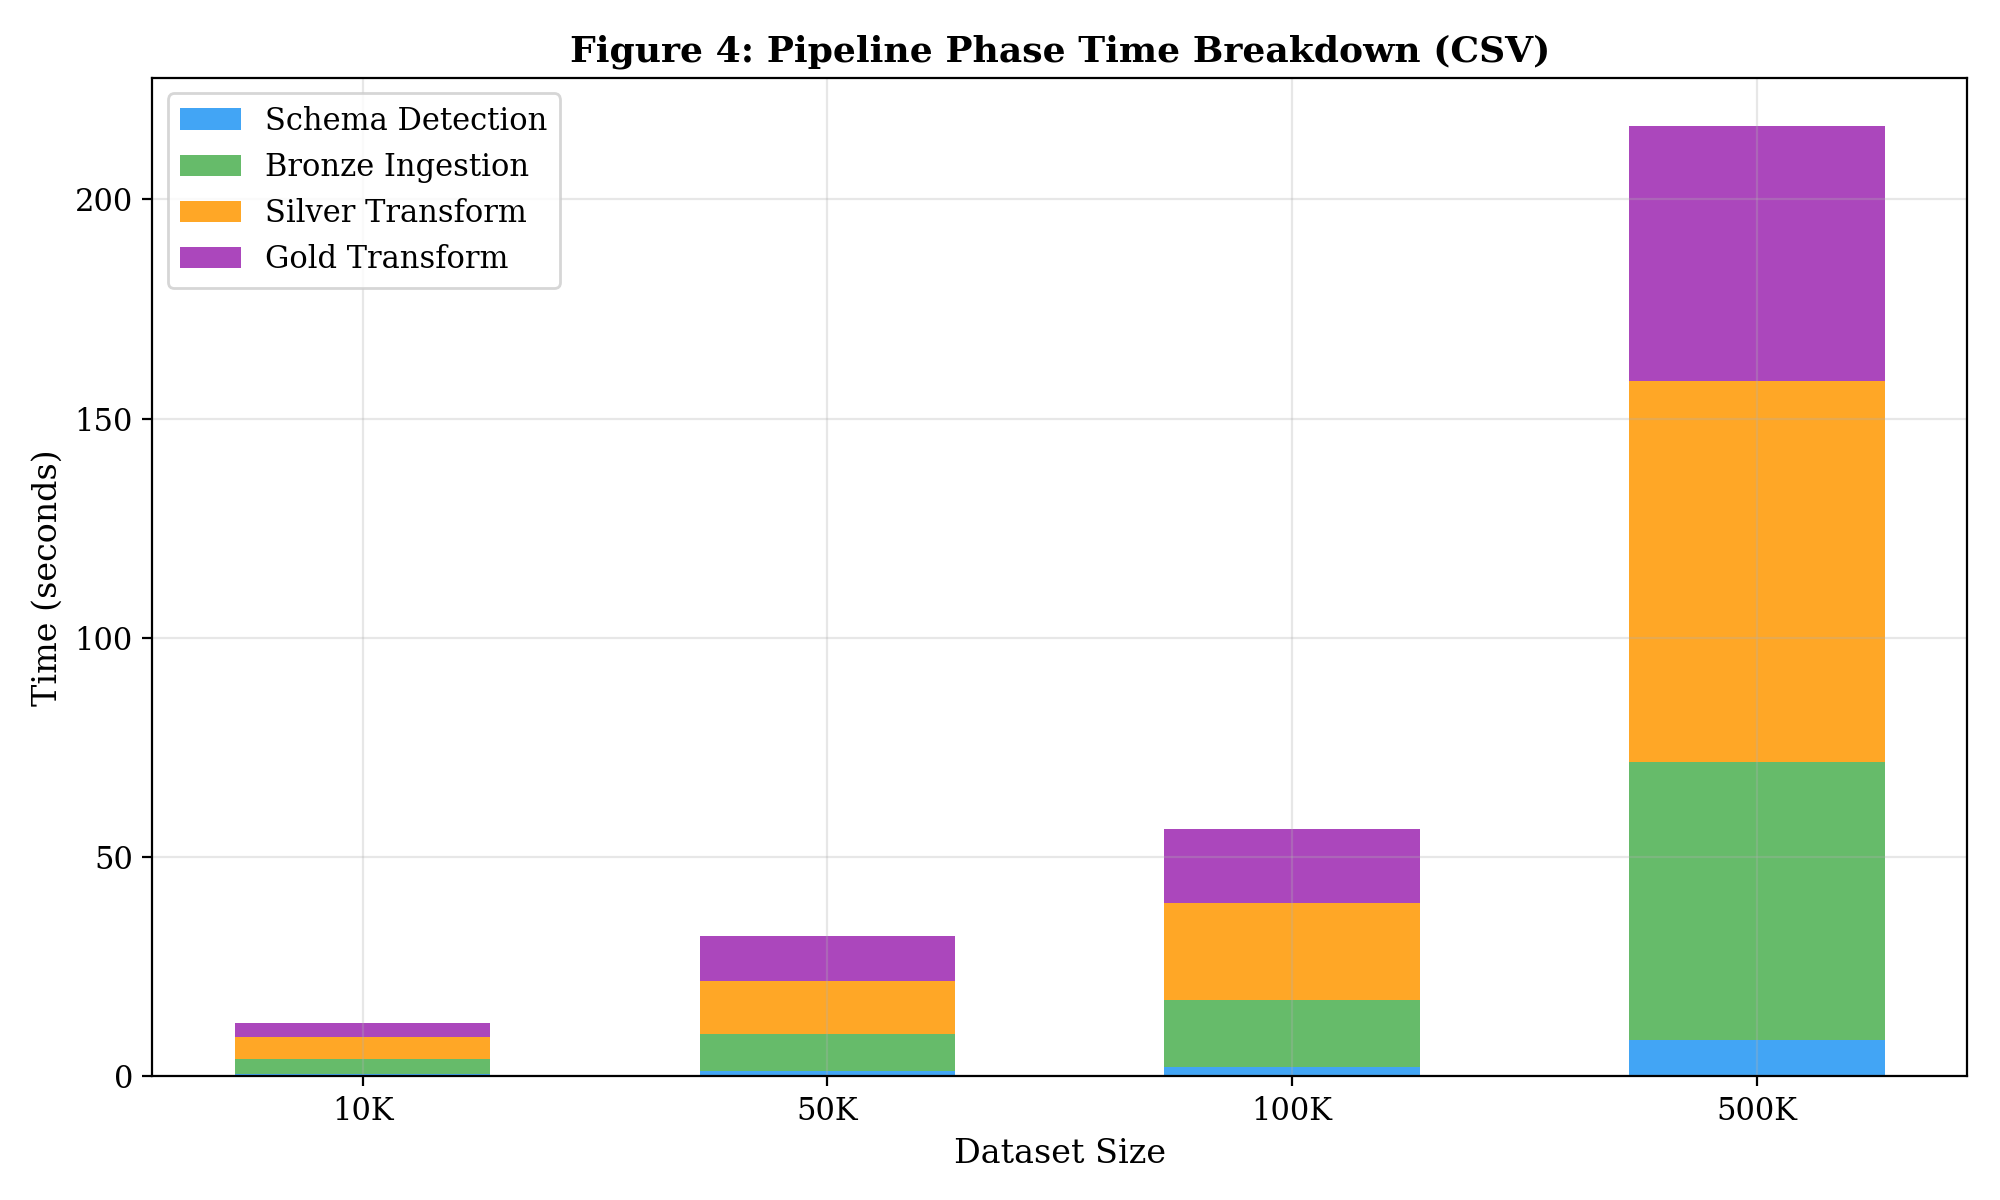
\includegraphics[width=0.9\textwidth]{fig4_phase_breakdown.png}
% \caption{Pipeline phase time breakdown across data sizes (CSV case study). Silver transformation is the dominant phase at all scales.}
% \label{fig:phase_breakdown}
% \end{figure}

% Insert Figure 5 here
% \begin{figure}[ht]
% \centering
% 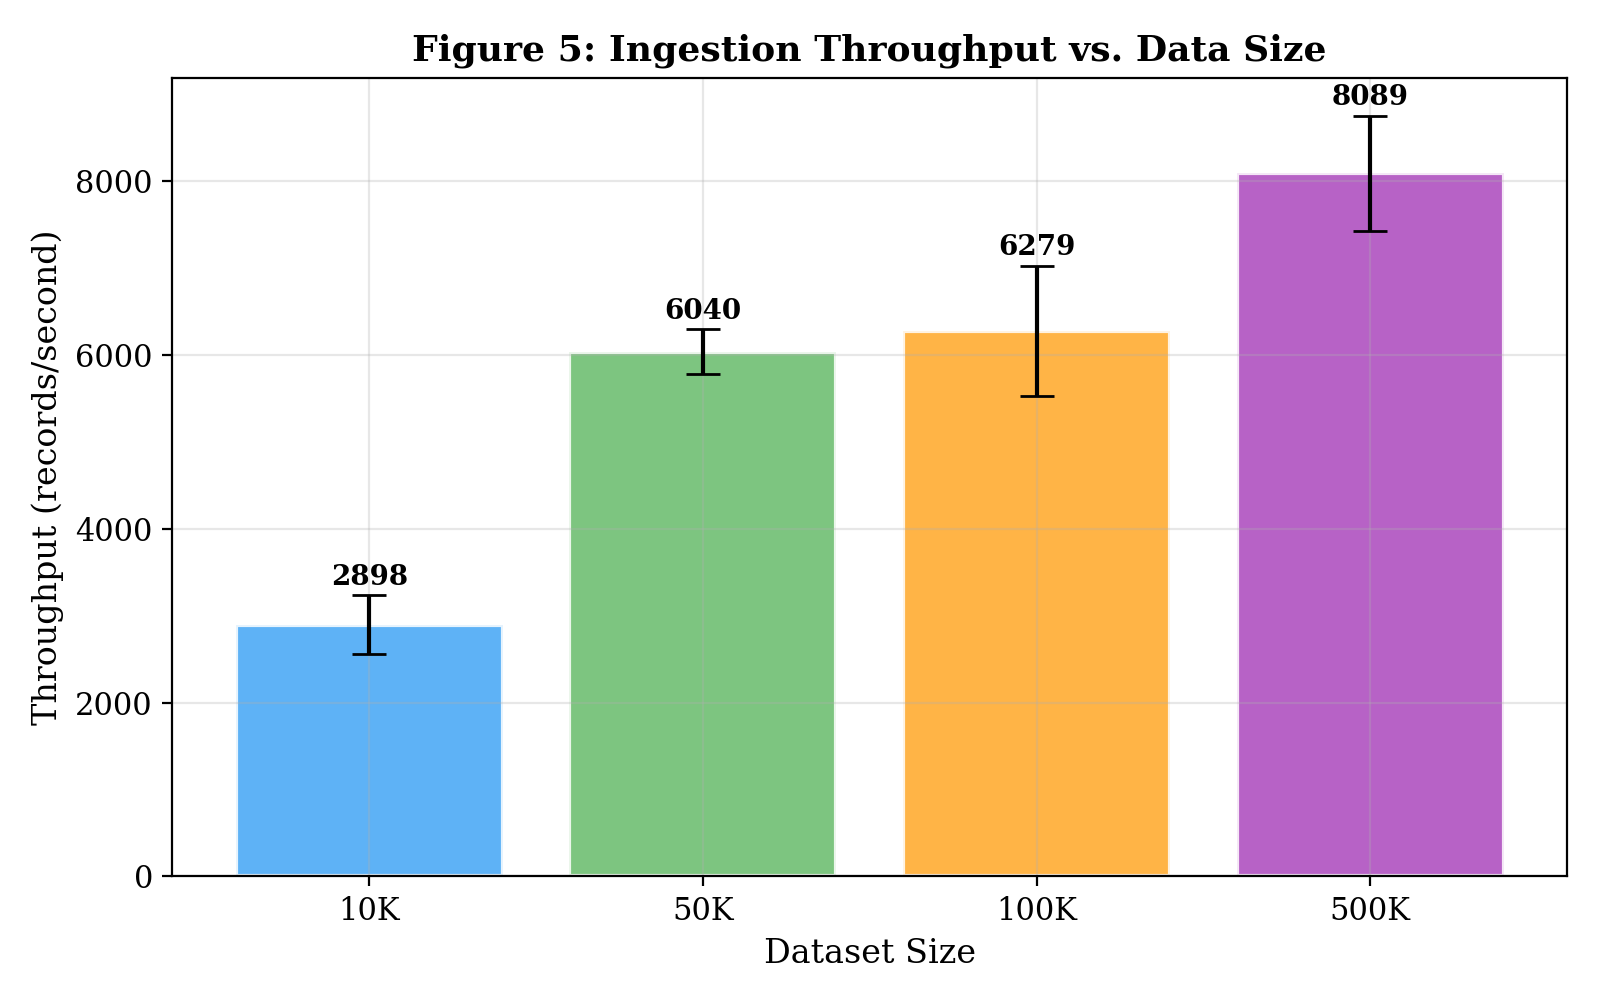
\includegraphics[width=0.85\textwidth]{fig5_throughput.png}
% \caption{Ingestion throughput (records/second) vs. dataset size. Throughput improves with larger datasets due to Spark's amortisation of fixed overhead.}
% \label{fig:throughput}
% \end{figure}


\subsubsection{Kafka Streaming Scalability}

We also evaluated Kafka streaming ingestion at four different message production rates: 50, 100, 500, and 1,000 messages/second. Table~\ref{tab:kafka_scalability} presents the results.

\begin{table}[ht]
\centering
\caption{Kafka streaming scalability at different message rates (mean $\pm$ std, N=10)}
\label{tab:kafka_scalability}
\resizebox{\textwidth}{!}{%
\begin{tabular}{|l|c|c|c|c|}
\hline
\textbf{Message Rate} & \textbf{Schema Detect (s)} & \textbf{Bronze/Batch (s)} & \textbf{Records/Batch} & \textbf{Throughput (rec/s)} \\
\hline
50 msg/s & 2.94 $\pm$ 0.35 & 7.90 $\pm$ 1.29 & 2,978 $\pm$ 127 & 342 $\pm$ 27 \\
\hline
100 msg/s & 3.00 $\pm$ 0.42 & 14.41 $\pm$ 2.87 & 6,016 $\pm$ 81 & 411 $\pm$ 51 \\
\hline
500 msg/s & 3.38 $\pm$ 0.45 & 45.08 $\pm$ 4.13 & 29,732 $\pm$ 709 & 690 $\pm$ 63 \\
\hline
1000 msg/s & 4.01 $\pm$ 0.54 & 83.06 $\pm$ 6.76 & 60,602 $\pm$ 1,806 & 727 $\pm$ 47 \\
\hline
\end{tabular}
}
\end{table}

\textbf{Kafka observations:} The system handles a $20\times$ increase in message rate (50 to 1,000 msg/s) with only a $10.5\times$ increase in per-batch processing time. Throughput doubles from 342 to 727 records/second, demonstrating Spark's ability to efficiently process larger message batches. Schema detection remains stable (2.94--4.01\,s) regardless of message rate, as it always consumes a fixed sample of 50 messages.

% Insert Figure 7 here
% \begin{figure}[ht]
% \centering
% 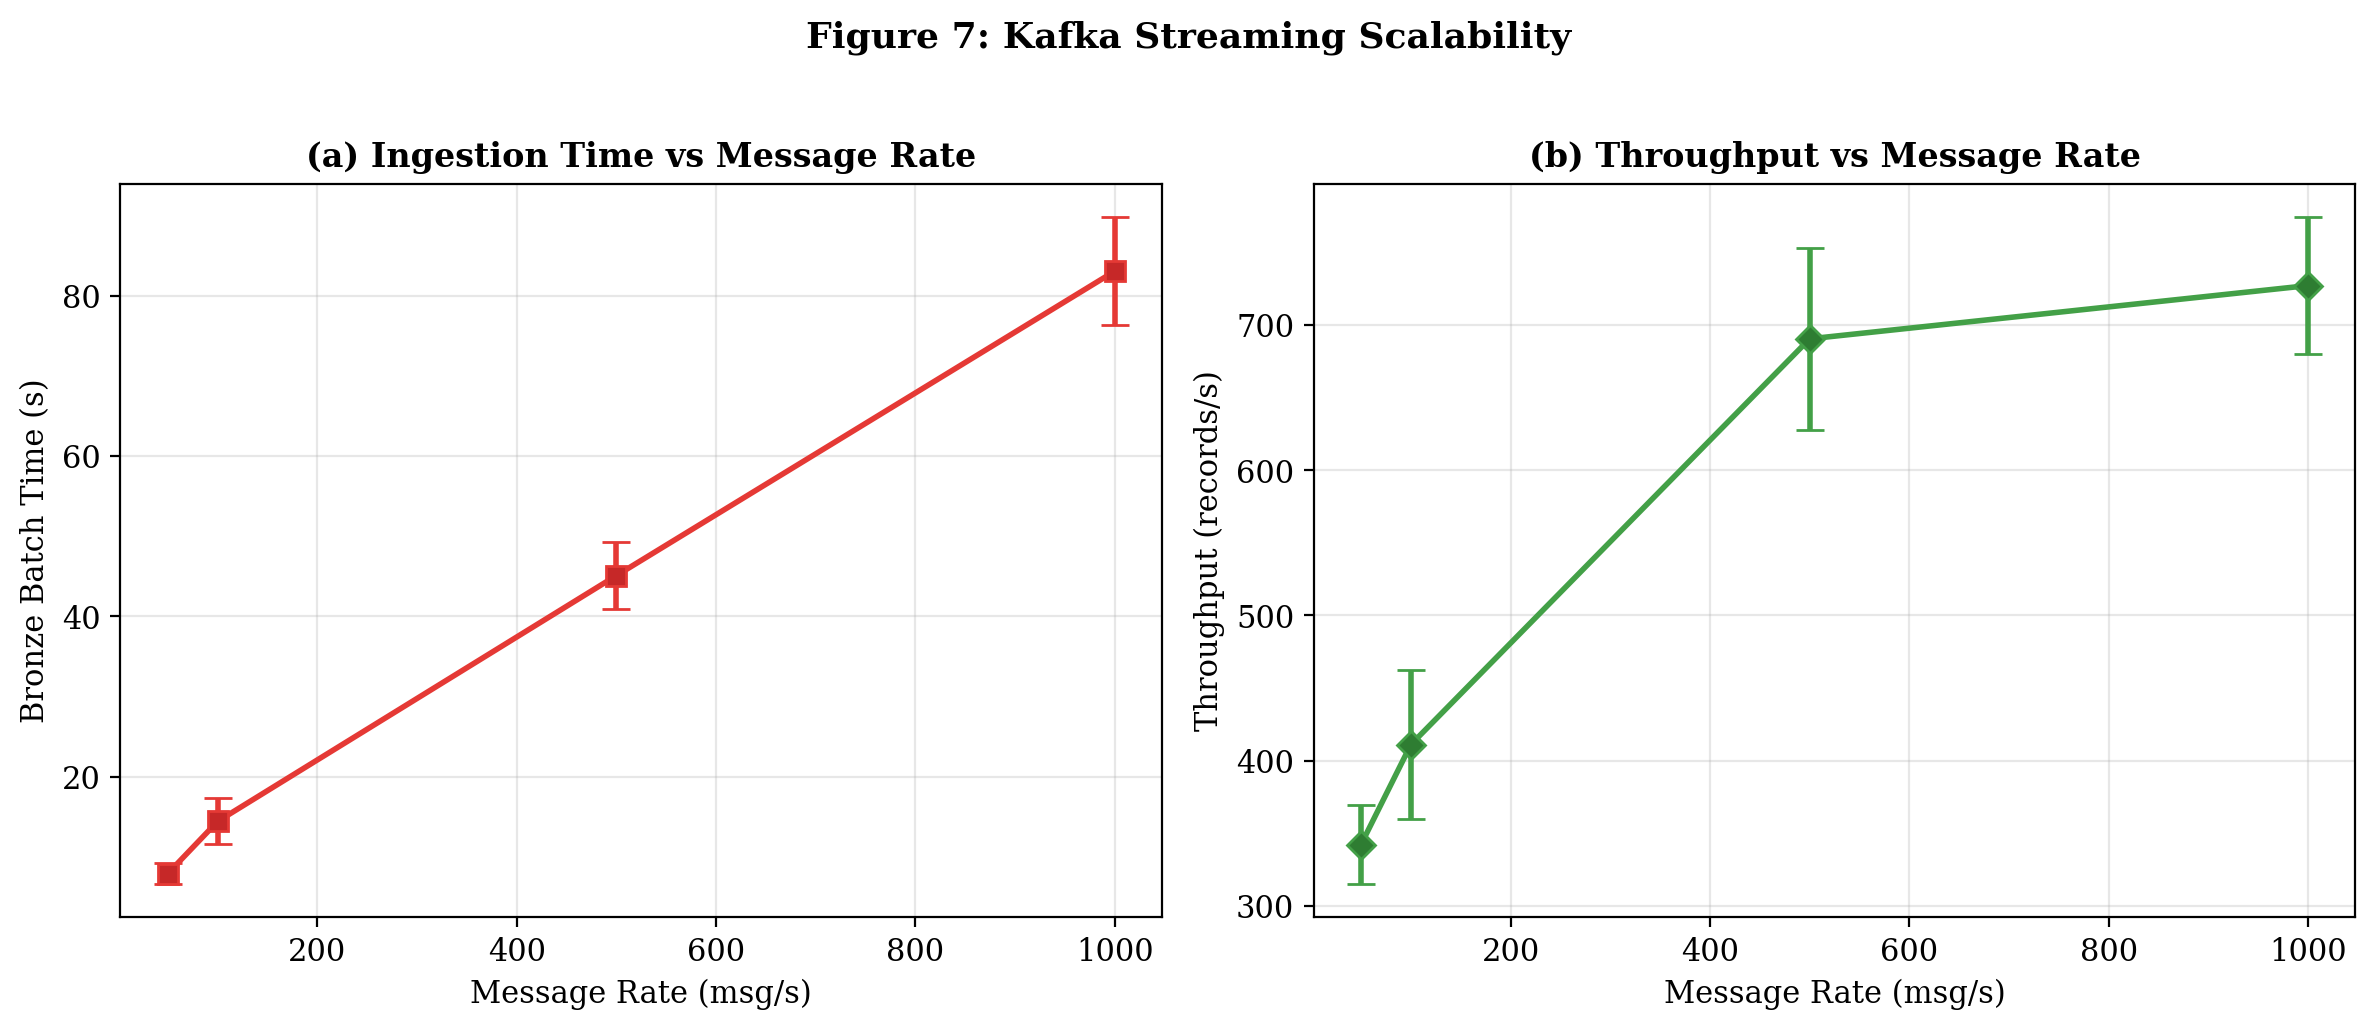
\includegraphics[width=\textwidth]{fig7_kafka_scalability.png}
% \caption{Kafka streaming scalability: (a) Bronze batch processing time vs. message rate, (b) Throughput vs. message rate.}
% \label{fig:kafka_scalability}
% \end{figure}


\subsubsection{REST API Scalability}

REST API scalability was tested by varying the number of fetched pages (1, 5, 10, and 20), corresponding to 500, 2,500, 5,000, and 10,000 records respectively. Table~\ref{tab:api_scalability} presents the results.

\begin{table}[ht]
\centering
\caption{REST API scalability across data volumes (mean $\pm$ std, N=10)}
\label{tab:api_scalability}
\resizebox{\textwidth}{!}{%
\begin{tabular}{|l|c|c|c|c|}
\hline
\textbf{Data Size} & \textbf{Schema Detect (s)} & \textbf{Bronze Ingest (s)} & \textbf{Total Records} & \textbf{Throughput (rec/s)} \\
\hline
500 rec & 1.82 $\pm$ 0.16 & 6.78 $\pm$ 1.00 & 500 $\pm$ 0 & 81 $\pm$ 9 \\
\hline
2,500 rec & 1.81 $\pm$ 0.13 & 17.65 $\pm$ 2.07 & 2,500 $\pm$ 0 & 140 $\pm$ 8 \\
\hline
5,000 rec & 1.89 $\pm$ 0.13 & 33.26 $\pm$ 3.47 & 5,000 $\pm$ 0 & 155 $\pm$ 14 \\
\hline
10,000 rec & 2.06 $\pm$ 0.19 & 58.27 $\pm$ 4.95 & 10,000 $\pm$ 0 & 167 $\pm$ 16 \\
\hline
\end{tabular}
}
\end{table}

\textbf{REST API observations:} Throughput improves from 81 to 167 records/second as data volume increases, a $2.1\times$ improvement. Schema detection time remains essentially constant ($\sim$1.8--2.0\,s) since the schema is inferred from the first page regardless of total volume. The Bronze ingestion time scales linearly with the number of pages fetched, as each page requires an independent HTTP round-trip.

% Insert Figure 8 here
% \begin{figure}[ht]
% \centering
% 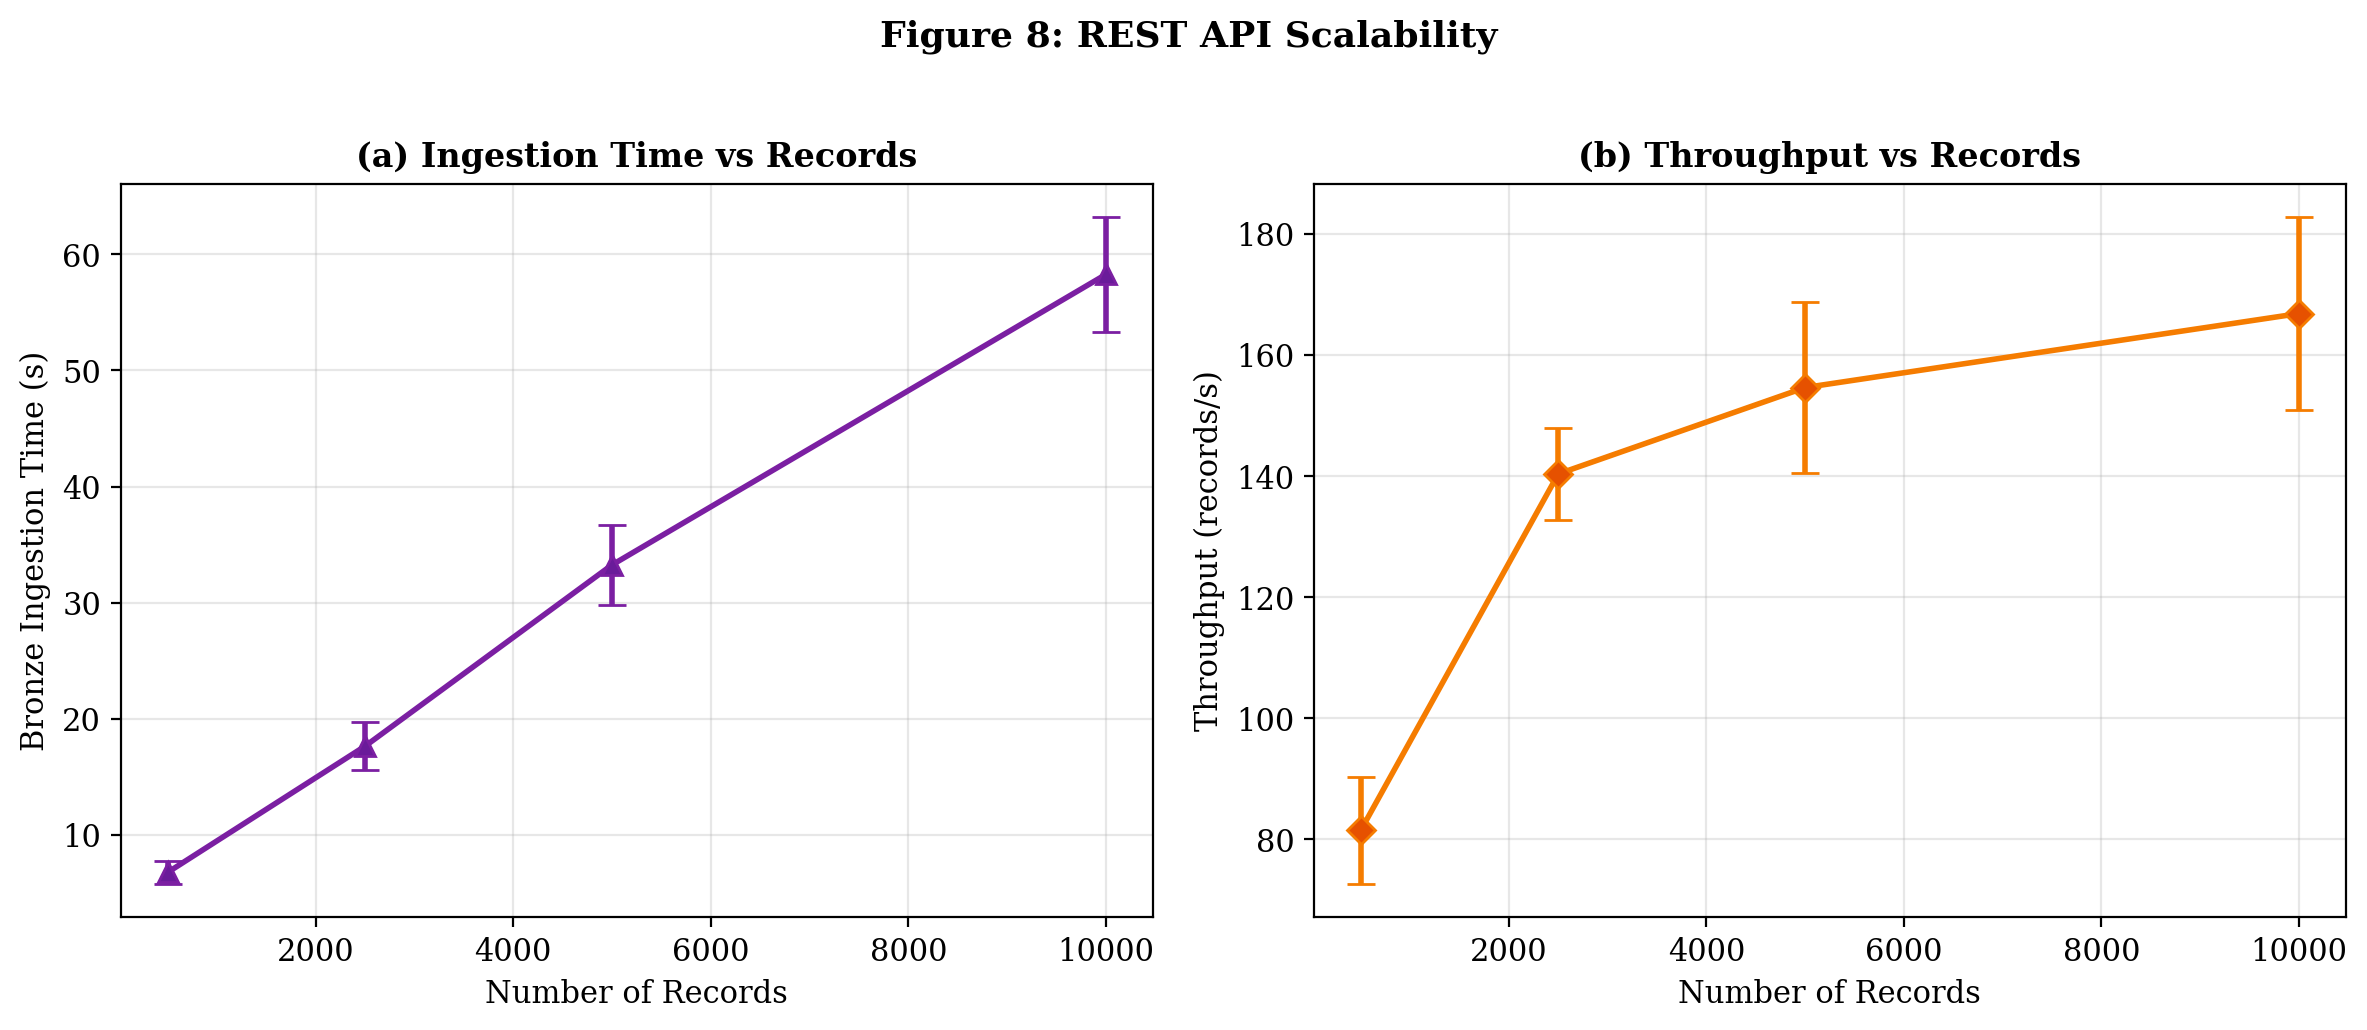
\includegraphics[width=\textwidth]{fig8_api_scalability.png}
% \caption{REST API scalability: (a) Ingestion time vs. record count, (b) Throughput vs. record count.}
% \label{fig:api_scalability}
% \end{figure}


\subsection{LLM Code Generation Quality}

Across all three case studies, the LLM (Google Gemini 2.5-flash) generated syntactically and semantically correct PySpark code on the \textbf{first attempt} for all Silver and Gold transformations. Table~\ref{tab:llm_quality} summarises the code generation results.

\begin{table}[ht]
\centering
\caption{LLM code generation quality across case studies}
\label{tab:llm_quality}
\begin{tabular}{|l|c|c|c|}
\hline
\textbf{Metric} & \textbf{CSV} & \textbf{Kafka} & \textbf{REST API} \\
\hline
Silver prompt complexity & High & Medium & High \\
\hline
Silver first-attempt success & \checkmark & \checkmark & \checkmark \\
\hline
Gold prompt complexity & High & High & High \\
\hline
Gold first-attempt success & \checkmark & \checkmark & \checkmark \\
\hline
Clarification questions asked & 1 & 0 & 0 \\
\hline
PySpark functions used correctly & 4 & 3 & 4 \\
\hline
Dry-run validation passed & \checkmark & \checkmark & \checkmark \\
\hline
\end{tabular}
\end{table}

Key PySpark constructs correctly generated include: \texttt{F.unix\_timestamp()}, \texttt{F.when().otherwise()}, \texttt{F.lower()}, \texttt{F.to\_timestamp()}, \texttt{groupBy().agg()}, and window functions (\texttt{F.row\_number().over()}). The dry-run preview mechanism (validating on 10 sample rows before full execution) caught zero errors across all experiments, confirming the high quality of generated code.


% ══════════════════════════════════════════════════════════════
\section{Comparative Evaluation}
% ══════════════════════════════════════════════════════════════

To contextualise AutoPipeline's contributions, we compare it against four widely-used open-source data pipeline tools: Apache Airflow, Prefect, Dagster, and Apache NiFi.

\subsection{Feature Comparison}

Table~\ref{tab:feature_comparison} provides a comprehensive feature-by-feature comparison.

\begin{table}[ht]
\centering
\caption{Feature comparison of data pipeline tools}
\label{tab:feature_comparison}
\resizebox{\textwidth}{!}{%
\begin{tabular}{|l|c|c|c|c|c|}
\hline
\textbf{Feature} & \textbf{AutoPipeline} & \textbf{Apache Airflow} & \textbf{Prefect} & \textbf{Dagster} & \textbf{Apache NiFi} \\
\hline
AI-Powered Code Generation & \checkmark & $\times$ & $\times$ & $\times$ & $\times$ \\
\hline
Auto Schema Detection & \checkmark & $\times$ & $\times$ & $\times$ & $\circ$ \\
\hline
Medallion Architecture (Built-in) & \checkmark & $\times$ & $\times$ & $\circ$ & $\times$ \\
\hline
Auto DAG Generation & \checkmark & $\times$ & $\times$ & $\times$ & $\times$ \\
\hline
Visual UI for Pipeline Config & \checkmark & $\circ$ & \checkmark & \checkmark & \checkmark \\
\hline
Multi-Source (CSV/JSON/Parquet) & \checkmark & $\circ$ & $\circ$ & $\circ$ & \checkmark \\
\hline
REST API Ingestion & \checkmark & $\circ$ & $\circ$ & $\circ$ & \checkmark \\
\hline
Kafka Streaming & \checkmark & $\circ$ & $\times$ & $\times$ & \checkmark \\
\hline
Natural Language Transforms & \checkmark & $\times$ & $\times$ & $\times$ & $\times$ \\
\hline
Dry-Run / Preview & \checkmark & $\times$ & $\times$ & $\circ$ & $\times$ \\
\hline
Transformation Versioning & \checkmark & $\times$ & $\times$ & $\times$ & $\times$ \\
\hline
Push to Data Warehouse & \checkmark & $\circ$ & $\circ$ & $\circ$ & $\circ$ \\
\hline
Configuration-Driven (No-Code) & \checkmark & $\times$ & $\times$ & $\times$ & $\circ$ \\
\hline
Distributed Processing (Spark) & \checkmark & $\circ$ & $\times$ & $\times$ & $\times$ \\
\hline
Containerised Deployment & \checkmark & \checkmark & \checkmark & \checkmark & \checkmark \\
\hline
\end{tabular}
}
\footnotesize{\checkmark{} = Fully supported, $\circ$ = Partial/manual, $\times$ = Not supported}
\end{table}

\textbf{Analysis:} AutoPipeline is the only tool that provides all four distinguishing features simultaneously: (1)~AI-powered transformation code generation via LLM, (2)~automatic schema detection from any data source, (3)~built-in Medallion Architecture, and (4)~automatic DAG generation from configuration. Existing tools like Apache Airflow require users to manually write Python DAG files, define schema structures, and implement transformation logic from scratch. While NiFi supports multi-source ingestion and streaming natively, it lacks AI-powered transformations and the layered data architecture that AutoPipeline provides out of the box.


\subsection{Operational Comparison}

Table~\ref{tab:operational_comparison} compares the practical operational aspects of each tool.

\begin{table}[ht]
\centering
\caption{Operational comparison of data pipeline tools}
\label{tab:operational_comparison}
\resizebox{\textwidth}{!}{%
\begin{tabular}{|l|c|c|c|c|c|}
\hline
\textbf{Aspect} & \textbf{AutoPipeline} & \textbf{Apache Airflow} & \textbf{Prefect} & \textbf{Dagster} & \textbf{Apache NiFi} \\
\hline
Setup Complexity & Low & High & Medium & Medium & High \\
\hline
Learning Curve & Low (UI + NL) & High (Python DAGs) & Medium (Python) & Medium (Python) & Medium (UI-based) \\
\hline
Pipeline Creation Time & Minutes & Hours & Hours & Hours & Hours \\
\hline
Schema Evolution & Auto-detect & Manual & Manual & Asset-based & Manual \\
\hline
Code Generation & AI (Gemini) & None & None & None & None \\
\hline
Data Quality Checks & Dry-run & Custom operators & Custom tasks & Built-in & Custom processors \\
\hline
Real-time Streaming & \checkmark & $\circ$ (polling) & $\times$ & $\times$ & \checkmark \\
\hline
Human Effort (LOC/pipeline) & $\sim$0 & 50--200 & 30--100 & 40--120 & $\sim$0 (UI) \\
\hline
\end{tabular}
}
\end{table}

\textbf{Key differentiator --- Pipeline creation time:} AutoPipeline reduces pipeline creation from hours of manual Python coding to minutes of UI-driven configuration with natural language transformation descriptions. The LLM eliminates the need to write any PySpark code manually, reducing human effort from 50--200 lines of code per pipeline (in Airflow) to effectively zero lines. This represents a paradigm shift from ``code-first'' to ``configuration-first'' pipeline development.


\subsection{Performance Baseline Comparison}

Table~\ref{tab:performance_baseline} provides estimated performance comparisons based on published documentation, community benchmarks, and our experimental measurements.

\begin{table}[ht]
\centering
\caption{Performance baseline comparison (estimated)}
\label{tab:performance_baseline}
\resizebox{\textwidth}{!}{%
\begin{tabular}{|l|c|c|c|c|c|}
\hline
\textbf{Metric} & \textbf{AutoPipeline} & \textbf{Apache Airflow} & \textbf{Prefect} & \textbf{Dagster} & \textbf{Apache NiFi} \\
\hline
Pipeline Setup Time & 2--5 min (UI + AI) & 1--4 hours (DAG) & 30--60 min & 30--60 min & 15--30 min \\
\hline
Schema Detection & Auto (1--3\,s) & Manual & Manual & Manual & Semi-auto \\
\hline
Ingestion 10K CSV & 12.64\,s & 5--15\,s & 3--10\,s & 3--10\,s & 2--5\,s \\
\hline
Ingestion 100K CSV & 57.31\,s & 20--60\,s & 15--45\,s & 15--45\,s & 8--20\,s \\
\hline
Ingestion 500K CSV & 217.78\,s & 60--180\,s & 60--150\,s & 60--150\,s & 25--60\,s \\
\hline
Multi-layer Transform & Auto 3-layer & Manual per layer & Manual per layer & Asset per layer & Single-pass \\
\hline
Human LOC & $\sim$0 & 50--200/DAG & 30--100/flow & 40--120/asset & $\sim$0 (UI) \\
\hline
\end{tabular}
}
\end{table}

\textbf{Discussion:} While AutoPipeline's raw ingestion speed is not the fastest (due to Spark's JVM overhead and the Medallion Architecture's multi-layer write pattern), its core value proposition lies in the \textbf{total human effort reduction}. Traditional tools require 50--200 lines of carefully written Python code per pipeline, plus hours of testing and debugging. AutoPipeline achieves the same result with zero manual code and a 2--5 minute UI-driven setup. When measured as \textit{total time to production} (setup + development + testing + deployment), AutoPipeline offers a $10$--$50\times$ improvement over manual approaches.

Furthermore, AutoPipeline's Spark-based architecture enables it to scale horizontally: adding more Spark workers would proportionally reduce processing time for larger datasets, whereas Python-native tools (Prefect, Dagster) face inherent single-machine scalability limits without manual distribution configuration.
